\subsection{Modelling}\label{sec:cloud:data_centers:modeling}
In this section, we first discuss the default data centre model, where a server can either be idle or busy, processing a job. Afterwards, the energy-efficient data centre model with the three states is defined.

\subsubsection*{Traditional Data Centre}\label{sec:cloud:data_centers:modeling:default}
We consider new jobs arriving at a \gls{POD} with exponential \gls{IID} inter-arrival times with rate \(\lambda\).
Each server accepts only one job at a time and processes it with an exponentially distributed service time with mean \(\frac{1}{\mu}\).
Then, the system can be modelled using a simple \(M/M/n\) delay system.
Here, the random variable \(X\) gives the number of jobs in the system and \(x(i)\) is the stationary probability that \(i\) jobs are currently in the system.

We obtain the mean power drain of such a system based on the measured values presented in \refsec{sec:cloud:data_centers:problem_formulation}.
If less than \(i < n\) jobs are currently in the system, then \(i\) servers are busy each consuming \(e_\text{busy}\) \si{\watt} and \(n-i\) servers are idle, where each consumes \(e_\text{idle}\) \si{\watt}.
If \(i \geq n\) jobs are in the system all servers are busy and consume \(n\cdot e_\text{busy}\) \si{\watt} in total.

Thus, for stationary state probabilities \(x(i)\), we obtain the mean power drain as
%TODO rename this
\begin{equation}\label{sec:cloud:data_centers:modeling:default:emax}
E_\text{max} = \sum_{i=0}^{n} x(i) (i e_\text{busy} + (n-i) e_\text{idle}) + ne_\text{busy} \sum_{i=n + 1}^{+ \infty} x(i).
\end{equation}

Furthermore, we can provide a lower bound for the power drain of the system by assuming that a server is turned off if it is not processing a job, thus consuming \(e_\text{off}\).
By substituting \(e_\text{off}\) for \(e_\text{idle}\) in \refeq{sec:cloud:data_centers:modeling:default:emax} we obtain
\begin{equation*}
E_\text{min} = \sum_{i=0}^{n} x(i) (i e_\text{busy} + (n-i) e_\text{off}) + ne_\text{busy} \sum_{i=n + 1}^{+ \infty} x(i).
\end{equation*}

\subsubsection*{Energy Efficient Data Centre}\label{sec:cloud:data_centers:modeling:energy_efficient}

We extend the queuing system to model the energy-efficient data centre model introduced in \refsec{sec:cloud:data_centers:problem_formulation}, by adapting the state space of the model.
We now model the system state as a tuple \((i,j)\) where \(i\) is gives the number of jobs currently in the system and \(j\) is \(1\) if the reserved servers are activated and \(0\) if they are not activated.
We give the state diagram in \reffig{fig:cloud:data_centers:modeling:energy_efficient:state_diagram}.
The system activates the reserved servers if more than \(\theta_2\) jobs are in the queue, i.e. more than \(n + \theta_2\) jobs are in the system.
The reserved servers are deactivated if the number of jobs in the system drops below \(\theta_1\).

Again, \(X\) is the random variable describing the number of jobs in the system if the reserved servers are activated or deactivated, and \(x(i, j)\) is the stationary probability that \(i\) jobs are in the system, and the reserved servers are activated, for \(j=1\), or deactivated, for \(j=0\). 

\begin{figure}
  \centering
  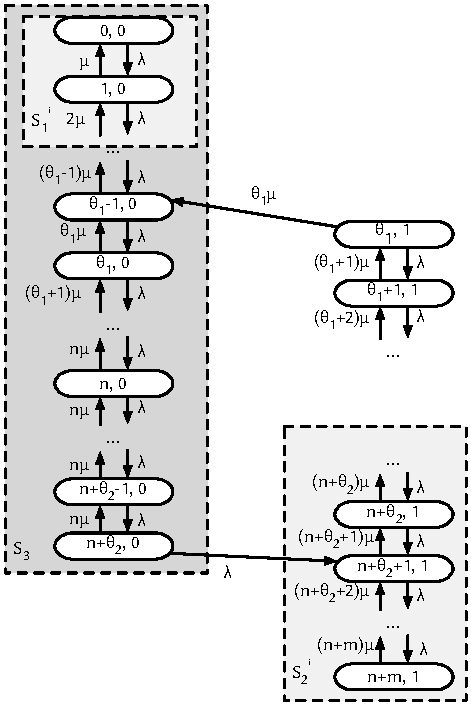
\includegraphics{cloud/data_centers/modeling/figures/state_diagram}
  \caption{\(M/M/(n+m)^{(\theta_1, \theta_2)}\) system with macro states \(S_1^i, S_2^i,\) and \(S_3\) for the calculation of \(x(i, \left\{0, 1\right\})\).}
  \label{fig:cloud:data_centers:modeling:energy_efficient:state_diagram}
\end{figure}

Based on the state space and transitions, we formulate macro state equations, defined as the sum of all local balance equations of the states contained in the macrostate.
They provide, when solved, the state probabilities required for further analysis. 

First,  we consider the macro state equations for state \(S_1^i\), which contains all system states where up to \(i-1\) jobs are in the system and no reserved servers are activated.
Depending on \(i\), we obtain the following equations
\begin{align}
i\mu x(i,0) &= \lambda x(i-1, 0) & 0<i<\theta_1\label{eq:cloud:data_centers:modeling:energy_efficient:S1_1}\\
i\mu x(i,0) + \theta_1 \mu x(\theta_1,1) &= \lambda x(i-1,0) & \theta_1\leq i\leq n\label{eq:cloud:data_centers:modeling:energy_efficient:S1_2}\\
n\mu x(i,0) + \theta_1 \mu x(\theta_1,1) &= \lambda x(i-1,0) & n\leq i\leq n+\theta_2\label{eq:cloud:data_centers:modeling:energy_efficient:S1_3}
\end{align}

Next, we examine the system state if the reserved servers are activated.
The macro state \(S_2^i\) contains all system states with activated reserved servers and at least \(i+1\) jobs in the system.
We get
\begin{align}
i\mu x(i,1) = \lambda x(i-1,1)\nonumber\\
 + \lambda x(n+\theta_2,0) && \theta_1<i\leq n+\theta_2+1\label{eq:cloud:data_centers:modeling:energy_efficient:S2_1}\\
 i\mu x(i,1) = \lambda  x(i-1,1) && n+\theta_2+1<i\leq n+m\label{eq:cloud:data_centers:modeling:energy_efficient:S2_2}\\
 (n+m)\mu x(i,1) =\lambda x(i-1,1) && n+m<i\label{eq:cloud:data_centers:modeling:energy_efficient:S2_3}
\end{align}

The third macro state \(S_3\) contains all system states where only the base-line servers are activated and its equation states
\begin{equation}
\lambda x(n+\theta_2,0) = \theta_1\mu x(\theta_1,1)\label{eq:cloud:data_centers:modeling:energy_efficient:S3}.
\end{equation}

Finally, the sum of all probabilities should be \(1\), i.e.
\begin{equation}
1=\sum_{i=0}^{n+\theta_2} x(i,0)+\sum_{i=\theta_1}^{+\infty}x(i,1)\label{eq:cloud:data_centers:modeling:normative}
\end{equation}
should hold.

Based on the state probabilities we can derive the required performance metrics for our analysis.

The carried traffic and utilisation is given by
\begin{equation*}
%TODO anders, evtl 2 zeilen?
a = \frac{\lambda}{\mu} \text{\quad and\quad} \rho=\frac{\lambda}{\mu(n+m)}.
\end{equation*}

Furthermore, we obtain the mean queue length
\begin{equation*}
\Omega = \sum_{i=n}^{n+\theta_2} (i-n)x(i,0) + \sum_{i=n+m}^{+\infty} (i-(n+m))x(i,1).
\end{equation*}
By applying macro state \refeq{eq:cloud:data_centers:modeling:energy_efficient:S2_3} we obtain for all \(i>n+m\)
\begin{equation}
x(i,1) = \rho x(i-1,1) = x(n + m,1)\rho^{i-(n+m)},
\label{eq:cloud:data_centers:modeling:x_i_redefinition}
\end{equation} 

Using this result and the first derivative of the geometric series we get 
\begin{eqnarray*}
\Omega &=& \sum_{i=n}^{n+\theta_2} (i-n)x(i,0) + x(n+m,1)\sum_{i=0}^{+\infty} i\rho^i\nonumber\\
&=& \sum_{i=n}^{n+\theta_2} (i-n)x(i,0) + x(n+m,1)\frac{\rho}{(1-\rho)^2}.
\end{eqnarray*}
Now, we can give the mean waiting time for all jobs in the system as
\begin{equation*}
E[W] = \frac{\Omega}{\lambda}.
\end{equation*}
Finally, we obtain the mean power drain similarly to \refeq{sec:cloud:data_centers:modeling:default:emax} as
\begin{align*}
E& = \sum_{i=0}^{n} x(i,0)(i e_\text{busy} + (n-i)e_\text{idle} + m e_\text{off})\\
&+ \sum_{i=n+1}^{n+\theta_2} x(i,0)(ne_\text{busy}+me_\text{off})\nonumber\\
&+\sum_{i=\theta_1}^{n+m} x(i,1)(i e_\text{busy} + (n+m-i)e_\text{idle})\nonumber\\
&+x(i > n+m)(n+m)e_\text{busy}.\nonumber
\end{align*}
